\input{./preamble.tex}

\newcommand*{\mytitle}{Generating Synthetic Images for Plant Disease in Sugar Beet using Augmentation Techniques} % Titel
\newcommand*{\myinstitute}{Department Lippstadt 2} % Institut


\newcommand*{\myauthor}{Olaniyi Bayonle Alao} % Autoren
\newcommand*{\myreporttype}{Bachelor Thesis} % Bericht-Typ
\newcommand*{\mygraduation}{Bachelor of Engineering} % Vollständige Anschrift



\newcommand*{\firstexaminer}{Prof. Dr. Stefan Henkler} % Ort
\newcommand*{\secondexaminer}{Prof. Dr. Achim Rettberg}
\newcommand*{\thirdexaminer}{Dipl.-Wirt.-inf. Kristian Rother} % Ort
\newcommand*{\mydate}{\today} % Datum



% ============= Dokumentbeginn =============

\begin{document}

% Seiten ohne Kopf- und Fußzeile sowie Seitenzahl
\pagestyle{empty}

\begin{center}
\begin{tabular}{p{\textwidth}}

\begin{center}
	\includegraphics[scale=0.12]{HSHL_Logo_horizontal_RGB_blue_green_mit-Schutzraum_ENG.jpg}
\end{center}


\\

\begin{center}
\LARGE{\textbf{
\mytitle\\[1cm]
}}
\end{center}

\\


\begin{center}
\large{\myinstitute\\}

\end{center}

\\\\

\begin{center}
\textbf{\Large{\myreporttype}}
\end{center}


\begin{center}
for optainment of the degree of\\
\mygraduation
\end{center}

\\\\

\begin{center}
submitted by
\end{center}

\begin{center}
\large{\textbf{\myauthor}} \\
% \small{geboren am 01.01.0001 in Entenhausen}
\end{center}

\\\\
\begin{center}


Electronic Engineering\\%name of study program
Mat.Nr.: 2180561\\
olaniyi-bayonle.alao@stud.hshl.de\\
\vspace{0.5cm}
\large{\mydate}


\end{center}

\\
\\
\\

\begin{center}
\begin{tabular}{lll}
\textbf{First supervisor:} & & \firstexaminer\\
\textbf{Second supervisor:} & & \secondexaminer\\
\textbf{Second supervisor:} & & \thirdexaminer\\
\end{tabular}
\end{center}

\end{tabular}
\end{center}	% Einbinden der Titelseite
\newpage 					% Um Seite nach der Titelseite einzubinden -> bei eigener Titelseite und nicht der Latex-Version erforderlich
\thispagestyle{empty}
\quad 
\newpage
\pagenumbering{Roman}
 
\cleardoubleoddpage

% ✅✅✅
\newpage
 \section*{Abstract}
This bachelor thesis aims to create synthetic leaf disease image datasets for sugar beet from available public datasets using image augmentation techniques. The lack of public image datasets for training disease detection models in sugar beet motivated this research. In order to create the synthetic dataset, we used publicly available sugar beet plant seedlings dataset and 
diseased image dataset of a plant that shares the same genus with a known disease in sugar beet from the PlantVillage dataset. 
We need to concatenate the extracted diseases in other plants to leaf areas of healthy seedling images of sugar beet plants. First, we will build a pipeline that can automatically overlay diseased areas on healthy areas of leaf images. Then, we present and evaluate the resulting images of the experiment by training convolutional neural network-based models. The experiment showed promising results to form a basis for further research on synthetic image generation for training disease detection models.
Finally, the thesis was concluded with a comprehensive overview of the chapters and discussed limitations encountered during the experiment with recommendations for future works.





\tableofcontents			%Inhaltsverzeichnis
% \onehalfspacing



%\chapter*{Abkürzungsverzeichnis}
%	\begin{acronym}[4GDH]	% Zur Formatierung hier die längste Abkürzung des Verzeichnisses eintragen
%		\acro{4GDH}{4th Generation District Heating} 	
%	\end{acronym}

\pagestyle{fancy}

\chapter{Introduction}
\label{cha:Introduction}
\pagenumbering{arabic}

% In the following I will explain in detail the introduction to the topic. In Section \ref{sec:Motivation} I will give a motivation on the thesis topic. Section \ref{sec:Goals} gives an overview of the goals this thesis and in Section \ref{sec:Overview} I will give an overview of my thesis. 


% ✅✅✅✅✅
% \section{Motivation}
% \label{sec:Motivation}
Currently, in the 21st century, computers have become ubiquitous in our everyday lives. Previously mundane tasks like switching on/off light switches, vacuuming, counting objects, and accurately predicting sales, to safety-critical tasks like driving vehicles and trains are currently performed efficiently by computers. Efforts are being made to extend the capabilities of computer systems to perform more intelligent tasks like disease detection, speech-to-text transcribing, anomaly detections that humans otherwise perform. However, the challenging part is transferring human knowledge to computers to perform such analysis and inference tasks. The approach humans use in learning is by transferring knowledge of a system to another related system. For example, humans can effortlessly differentiate between a cat and a dog in an image. This ability to differentiate is possible because specific characteristics are present in dogs but absent in cats, irrespective of their breeds. However, manually programming computers to make such differentiation will prove impractical or possibly amount to several lines of code. Likewise, it is unrealistic to manually program a computer to detect diseases in an image or make driving decisions in the case of autonomous vehicles. 

These shortcomings for computers have motivated researchers to trial the use of machine learning techniques to allow computers to analyse and interpret objects in images or videos. An exciting use case in agriculture is training models to monitor and detect plant leaf diseases or nutrient deficiencies through image data. The use of computers to precisely monitor and give respective treatment to particular plants in plantations to get increased average yields and reduce operational farming costs is known as precision farming. 

Traditionally, disease detection techniques used to involve using naked eyes to visually inspect the leaves and branches of plants for any sign of infection. However, this plant health monitoring and disease detection method are time-consuming. For example, it is labour tasking and financially draining to visually inspect plant leaves spanning several hectares of land. Thanks to the advancements in the technological sector, researchers have shown the possibilities of plant health monitoring using machine learning techniques to classify plant leaves captured with RGB (Red Green Blue) cameras and hyperspectral sensors as healthy or unhealthy. Unfortunately, one major challenge in using these technologies is the unavailability of sufficient datasets for model training.




% ✅✅✅✅
\section{Goals}
\label{sec:Goals}
Plant diseases cause significant hindrances to the sustainability and profitability of agriculture \cite{harvey2014extreme}. In order to prevent the losses that come with diseases in plants, different methods have been developed to monitor and diagnose these diseases before they lead to a significant infestation. One of such methods is the use of established knowledge in molecular biology and immunology to precisely identify the causal agents of diseases in plants and develop treatments for eradicating them before they become catastrophic to the plants. However, such an approach requires experts in the disease domain to cut down the plants and perform tests to identify the specific disease affecting the plants. Moreover, this disease detection technique is invasive; it is likewise tedious and expensive \cite{wang2017automatic}.

These shortcomings in the traditional disease detection motivated research in the direction of non-invasive plant disease detections using data from sensors like RGB, hyperspectral imaging and spectroscopy with machine learning algorithms \cite{mohanty2016using, ashourloo2016investigation, zhang2019deep}. The research results on the use of collected real-time data from plants with machine learning techniques showed promising results that are more accurate in plant disease detection and classification than domain experts in such fields, thereby potentially minimising costs for farmers \cite{barreto2020hyperspectral}. 
Standard algorithms used for plant disease detection and classification tasks are linear regression, logistic regression, random forest, clustering, Gaussian models, decision trees (DT), Naïve Bayes (NB), K-nearest neighbours (KNN), and support vector machines (SVM) among others.


Despite the success of plant disease detection, using sensor data with classical machine learning (ML) algorithms was time-consuming due to manual feature extractions and not being robust enough for use on datasets containing variations from the original training dataset \cite{ferentinos2018deep}. Nevertheless, the understandings from ML laid a solid foundation for current research in the direction of deep neural networks for automating the identification of disease from the data captured from sensors to allow precise plant treatment in a field. Furthermore, advancements in computer vision and artificial intelligence have led to solutions that were found to accurately solve complex decision-making tasks like yield forecasting \cite{liu2017computer}, plant recognition \cite{gao2017mobile}, and nutrition deficiency \cite{yi2020deep} in precision farming.

Consequently, deep neural networks require a large amount of image data with appropriate diversity representing different conditions that can likely occur to create a high-quality model for the trained tasks. However, capturing all the variability of conditions possible is a cumbersome task, hence the need to augment the existing dataset using computer vision and deep learning techniques to create robust image datasets for plant disease detection tasks in sugar beet. Furthermore, there are no publicly accessible datasets for sugar beet disease detection, and acquiring these datasets requires several months and professionals to ensure the quality and diversity needed \cite{barreto2020hyperspectral, jay2020scoring}.
% [\cite{} papers that it took them months to get sugar beets dataset].

This thesis proposes the approaches below to solve the lack of a publicly available dataset for disease detection in sugar beet plants: 
%Furthermore, understandings from this experiment can be utilised to create disease leaf images in other plants.
 \begin{itemize}
     \item Use image augmentation techniques to overlay diseased areas in a plant on top of healthy areas in another plant. However, there should be a common disease occurrence in both plants.
     \item Validate the generated images by training convolutional neural network (CNN) based disease detection models using the synthetic images and the original healthy sugar beet images.

 \end{itemize}


The results from creating these synthetic datasets will create an avenue for transferring knowledge in this domain to create more datasets for other plants, hence creating more than enough datasets for model training.

% ✅✅✅✅
\section{Sketch of Approach}
\label{sec:Overview}
% The required fundamentals of this thesis are explained in Chapter \ref{cha:Fundamentals}. These include the fundamental basics of automata theory. Related work is discussed in Chapter \ref{cha:RelatedWork}. The detailed consideration of the influences on this work, such as existing systems to be considered, user requirements and environmental influences, are analysed in Chapter \ref{cha:Analysis}. Based on this analysis as well as related work, a design is presented in Chapter \ref{cha:DesignImplementation} that considers the posed requirements of this work. An evaluation of the developed approach is presented in Chapter 6. Here, the requirements set are reflected upon. Finally, a summary and outlook is presented in Chapter \ref{cha:SummaryOutlook}.  

Our approach to artificial dataset creation is based on segmenting the leaf areas of the diseased and healthy plants from their background in the images and then concatenating the extracted diseased areas intelligently on the healthy leaf areas. First, we propose segmenting foreground and background leaf areas by converting the images to their respective HSV (Hue Saturation Value) values to find the leaves’ upper and lower bound values. We then propose using thresholding algorithms to create binary masks of the leaf areas and the background and finally use boolean operations to create the new image. Furthermore, we propose bringing the infected areas of the diseased leaf to the foreground and then masking out healthy areas to become the background. Figure \ref{fig:my_arch} showcases a visual representation of the proposed artificial dataset creation pipeline. 
% The values corresponding to the diseased areas are rotated and placed accordingly on the leaf areas of the sugar beet plants, as shown in figure \ref{fig:my_arch}.
The extracted disease areas in the left side of figure \ref{fig:my_arch} are concatenated with segmented healthy leaf areas of sugar beet in the right side of the figure to create synthetic disease images.

\begin{figure}[!htb]
    \centering
    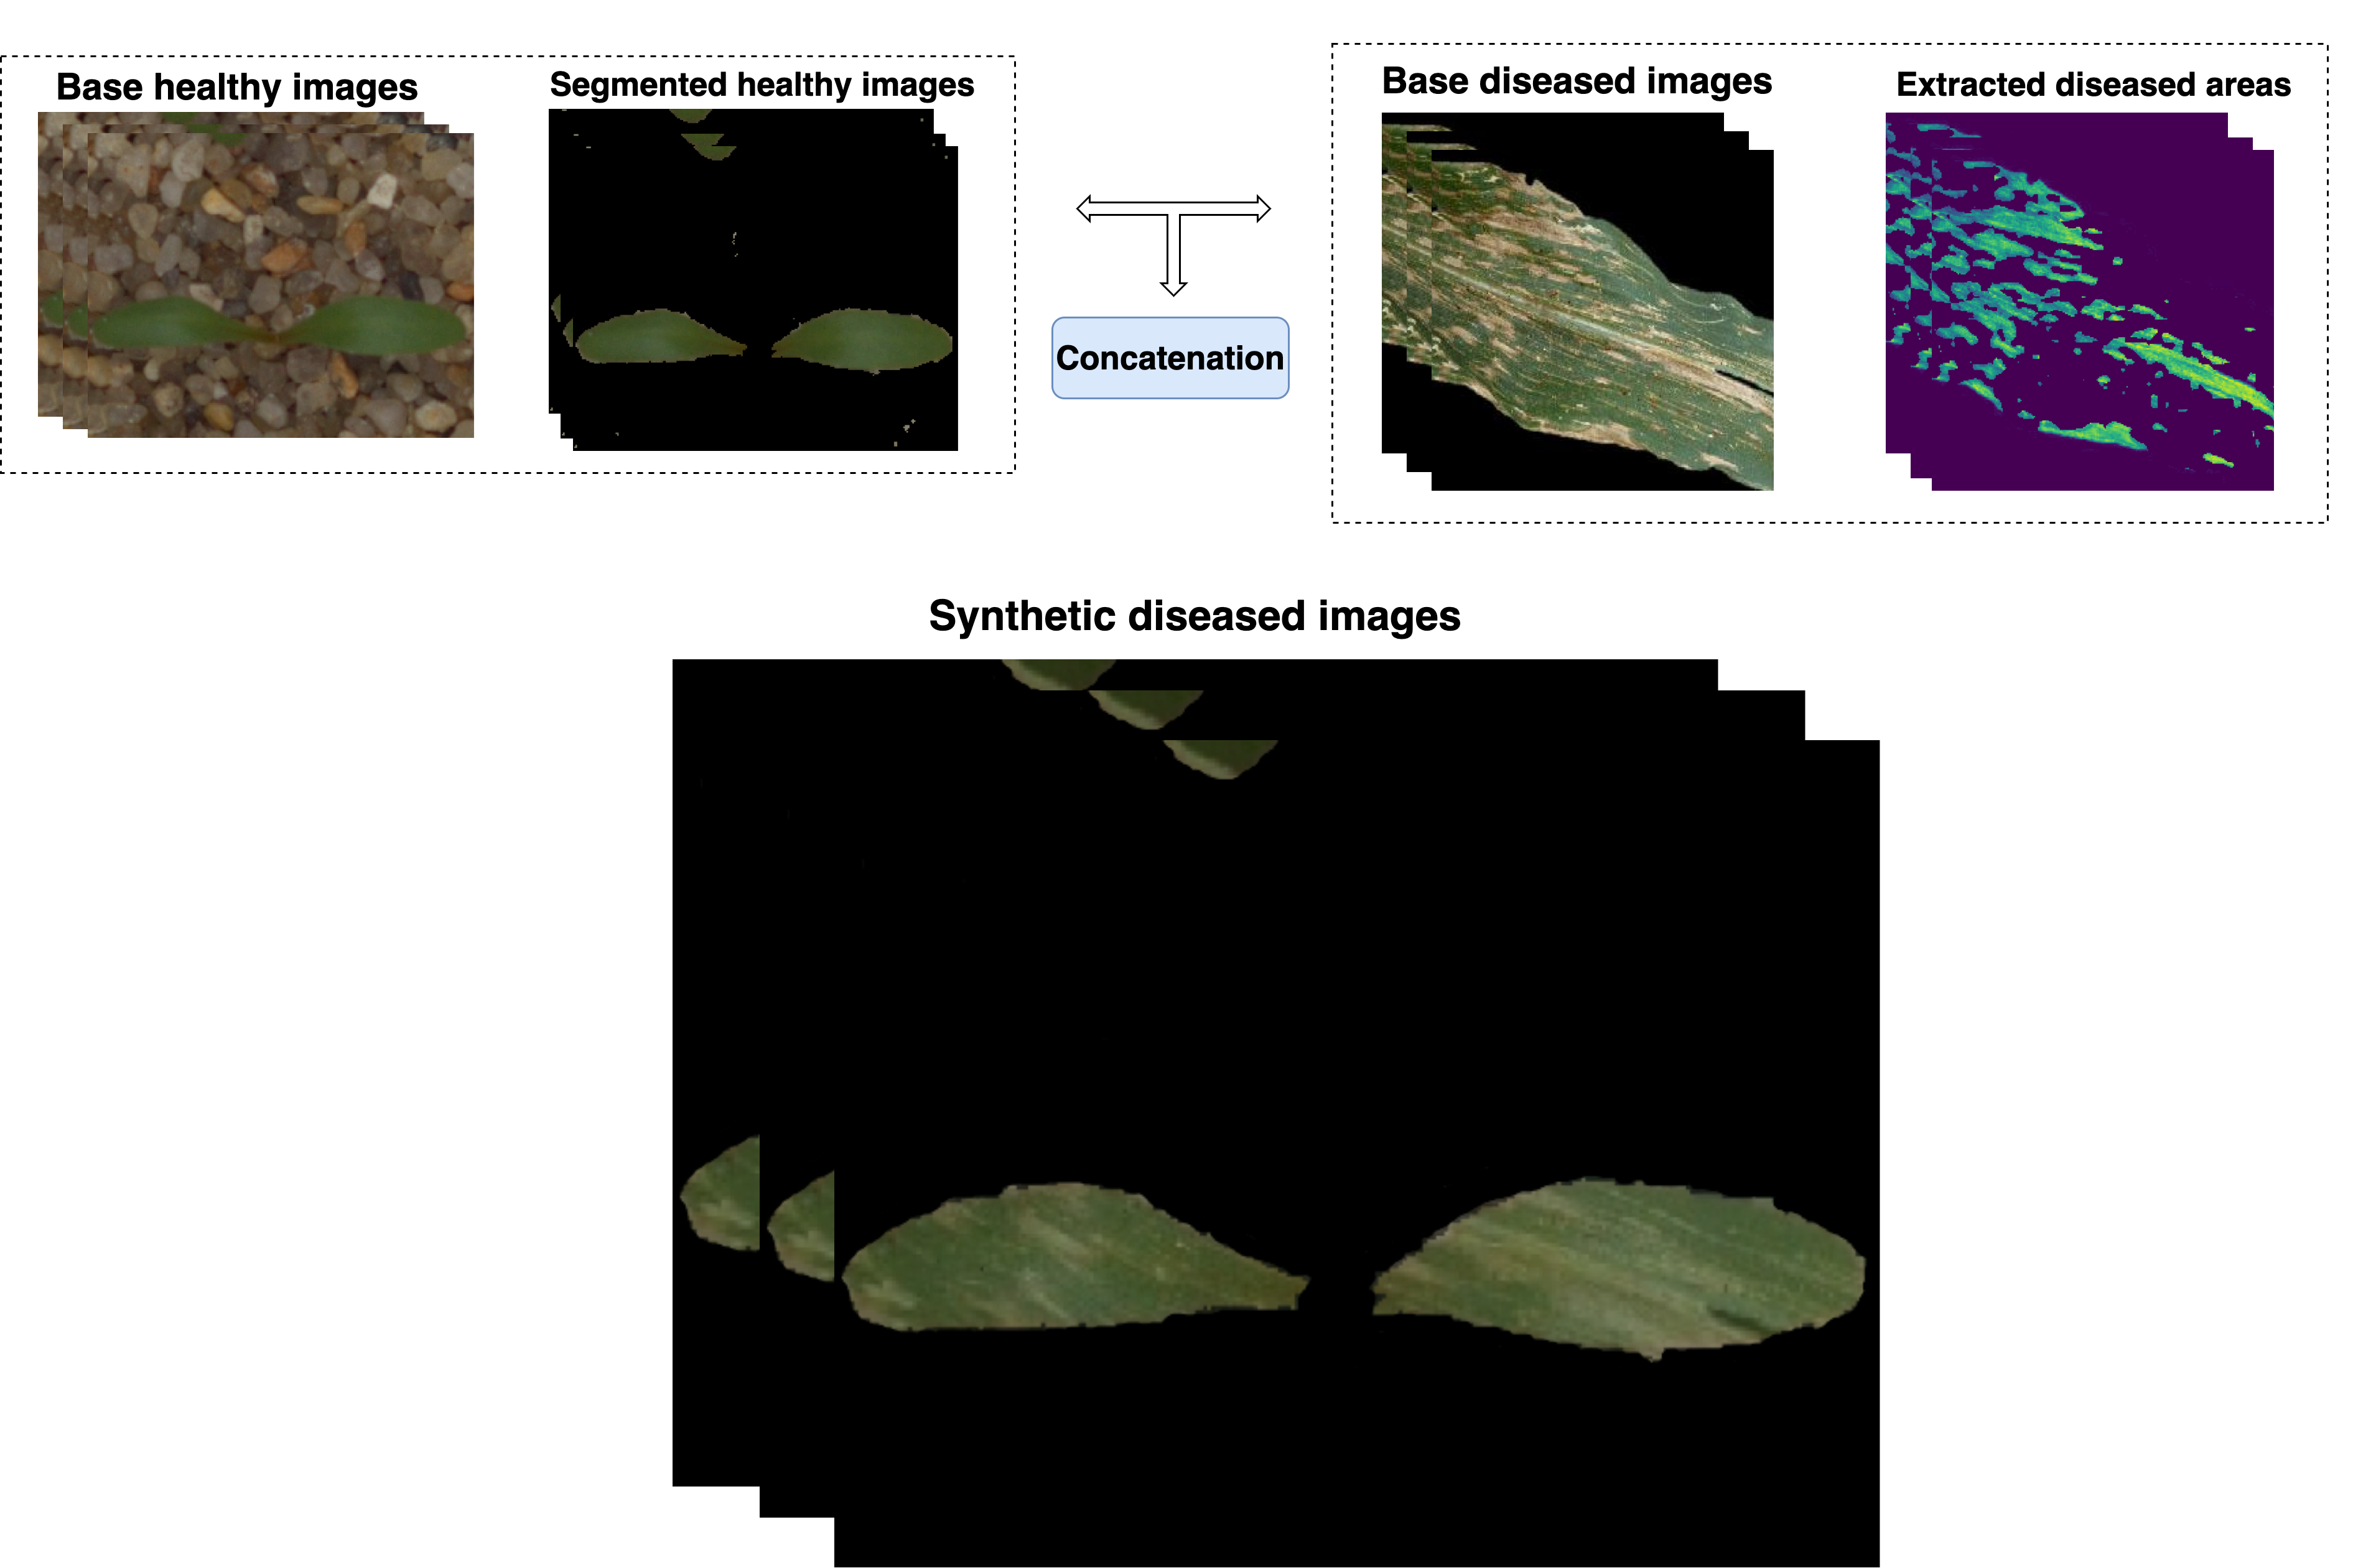
\includegraphics[width=1\textwidth]{Figures/architecture.png}
    \caption{Overview of proposed appraoch for generating artificial dataset.}
    \label{fig:my_arch}
\end{figure}

With the resulting images from the previously proposed approach, we suggest potentially automating the process of creating more randomly unique datasets using generative adversarial neural networks (GAN). On a high level, GANs work by using two neural networks competing against each other to create synthetic datasets. First, the neural generator network creates new synthetic image data, which are then fed to the discriminator neural network to ascertain how close the generated image is to the original images.

\section{Organisation of Paper}

In section \ref{sec:Goals}, we described plant disease monitoring and disease detection and the goals of the thesis to address the lack of sufficient datasets for model training. Then, in section \ref{sec:Overview} we gave an overview of the sketch of approaches for implementing the proposed approach to solving the lack of public dataset in sugar beet for disease detection tasks. Next, chapter \ref{cha:Fundamentals} explains the relevant fundamentals necessary for the experiment performed in this research. Then, in chapter \ref{cha:RelatedWork} we highlight related works to the thesis. Next, based on the knowledge from the related works and fundamentals described in previous chapters, chapter \ref{cha:DesignImplementation} presents the prerequisites and a high-level overview of the approach design and its implementation. Next, chapter \ref{cha:Evaluation} presents and discusses the results of the generated synthetic image datasets. Finally, chapter \ref{cha:SummaryOutlook} concludes the research work by summarising the thesis and giving recommendations for future work. 

% \begin{itemize}
    
%     \item \textbf{Chapter 2:} explains the relevant fundamentals necessary for the experiment performed in this research. 
%     % Furthermore, the chapter presents the related works to the thesis.

%     \item \textbf{Chapter 3:} highlights related works to the thesis.

%     \item \textbf{Chapter 4:} presents the prerequisites and a high-level overview of the approach design and its implementation

%     \item \textbf{Chapter 5:} presents and discusses the results of the generated synthetic image datasets.

%     \item \textbf{Chapter 6:} draws a conclusion by summarising the thesis and giving recommendations for future work. 
    
% \end{itemize}

% This chapter introduces the problem of plant health monitoring using machine learning techniques. First, it discusses the issue of not having enough datasets to train machine learning algorithms for plant health monitoring - particularly the lack of public datasets for disease detection in sugar beets. Then the chapter continues by shortly presenting the proposed approach to solving the lack of public dataset in sugar beet for disease detection tasks, highlighting the contributions of the thesis. The rest of the thesis is structured as follows.

% \begin{itemize}
    
%     \item \textbf{Chapter 2:} explains the relevant fundamentals necessary for the experiment performed in this research. 
%     % Furthermore, the chapter presents the related works to the thesis.

%     \item \textbf{Chapter 3:} highlights related works to the thesis.

%     \item \textbf{Chapter 4:} presents the prerequisites and a high-level overview of the approach design and its implementation

%     \item \textbf{Chapter 5:} presents and discusses the results of the generated synthetic image datasets.

%     \item \textbf{Chapter 6:} draws a conclusion by summarising the thesis and giving recommendations for future work. 
    
% \end{itemize}%link to chapters
\chapter{Fundamentals}
\label{cha:Fundamentals}	
This chapter explains the relevant fundamentals necessary for the experiment performed in this research. 

% ✅✅✅✅✅✅
\section{Digital Image Formation}
A digital image is a two-dimensional pixels array(matrix) composed of picture elements. Each pixel represents the numeric representation of the brightness of the corresponding picture element in the x and y-axis. Furthermore, a digital colour image stores colour information for each pixel in three intensity components (channels). A pixel in a colour image represents the value of the combination of three colours Red, Green, and Blue (RGB). Standard formats of storing the colour information are RGB (red, green, blue channels), HSV or HSB (hue, saturation, brightness) and YCbCr (where Y is the luma component, Cb and Cr are the blues and red components relative to the green component). For example, an RGB image supports 16,777,216 different colours because each channel occupies a maximum of 8-bit colour variations (i.e. between 0 and 255). A digital image can be converted from one colour space to another for easy manipulation purposes. 


% ✅✅✅✅✅
\section{Grayscaling}
A grayscale image is a black and white image with shades of grey in-between. There are different techniques for converting a colour image to grayscale. 

\cite{pratt2007digital} developed a color to grayscale image technique using weighted combination of RGB channels in equation \ref{lumi_eqn}. Also, a colour image can be grayscaled using equation \ref{value_eqn} by taking the maximum of the RGB channels \cite{acharya2005image} or taking the average of the three channels \cite{jack2007ntsc} as denoted in equation \ref{inten_eqn}.

\begin{equation} \label{value_eqn}
G_{value} = \max (R,G,B)
\end{equation}

\begin{equation} \label{lumi_eqn}
G_{luminance} = 0.3R + 0.59G + 0.11B
\end{equation}
\begin{equation} \label{inten_eqn}
G_{intensity} = \frac{R +G+B}{3}
\end{equation}
Using grayscale images for extracting descriptors is computationally cheaper and simplifies the algorithm compared to colour images due to working with only one channel (luminance information) as compared to three channels in colour images \cite{kanan2012color}. For example, a 24-bit RGB image becomes 8-bit when converted to grayscale. However, the above mentioned and other colours to grayscale algorithms have different time computation, and appropriate use case scenarios in image recognition tasks \cite{cadik2008perceptual}. According to Kanan and Cottrell \cite*{kanan2012color}, equation \ref{lumi_eqn} is good for object and face recognition tasks.

% ✅✅✅✅✅
\section{Thresholding}
Thresholding is a popular and computationally straightforward technique in computer vision for foreground and background segmentation of images \cite{lee1990comparative}. Thresholding works by converting grayscale images to binary images according to the pixels’ threshold value \cite{nixon2019feature}. This means that each pixel’s brightness/grey value in the interested objects/regions of the input image must be known. The grey values of objects and background can be obtained by drawing a grayscale image histogram.
As the operator of the threshold algorithm goes through every pixel in the image, if the value of the respective pixel is greater than the threshold, it is set to the maximum pixel value (255, i.e. white). On the other hand, if the pixel value is less than the threshold, the value is set to (0, i.e. black). Hence the final image becomes a white and black image showing a segmented region of interest. For example, figure \ref{fig:my_place} shows a thresholded image, where the original image (a) has been transformed into a grayscale image (b), and (c) is a thresholded image where all pixels above the value of 150 are set to 255 and pixels below the threshold value are set to 0. 

\begin{figure}[!htb]
    \centering
    \includegraphics[scale=0.55, keepaspectratio]{Figures/notebook/thresholding.png}
    \caption{(a) Original image (b) Grayscale image (c) Thresholded image.}
    \label{fig:my_place}
\end{figure}  

Sezgin and Sankur \cite{sezgin2004survey} categorises thresholding operators based on the parameters used for manipulating grayscale images into the following six categories.

\begin{itemize}
\item histogram shape-based methods, in this method, the peaks, valleys and curvatures of the smoothed histogram are analysed.
\item clustering-based methods, where the grey-level samples are clustered in two parts as background and foreground objects, or alternately are modelled as a mixture of two Gaussians.
\item entropy-based methods result in algorithms that use the entropy of the foreground and background regions, the cross-entropy between the original and binarised image.
\item object attribute-based methods search a measure of similarity between the grey-level and the binarised images, such as fuzzy shape similarity edge coincidence.
\item the spatial methods use higher-order probability distribution and correlation between pixels.
\item dynamic/local methods adapt the threshold value on each pixel to the local image characteristics.

\end{itemize}

Furthermore, according to Guruprasad \cite{guruprasad2020overview}, the main forms of thresholding methods are:
\begin{itemize}
    \item Threshold Binary
    
    \[
    K(x,y) = \Bigg|_{0 \qquad\quad otherwise}^{maxVal \quad if \quad L(x,y) > threshold}
    \]
    
    \item Threshold Binary, Inverted
    
    \[
    K(x,y) = \Bigg|_{maxVal \qquad\quad otherwise}^{0 \quad if \quad L(x,y) > threshold}
    \]
    
    \item Threshold to zero
    
    \[
    K(x,y) = \Bigg|_{L(x,y) \qquad\quad otherwise}^{0 \quad if \quad L(x,y) > threshold}
    \]
    
    \item Threshold to zero, Inverted
    
    \[
    K(x,y) = \Bigg|_{0 \qquad\quad otherwise}^{L(x,y) \quad if \quad L(x,y) > threshold}
    \]
    
    \item Truncate
    
    \[
    K(x,y) = \Bigg|_{L(x,y) \qquad\quad otherwise}^{threshold \quad if \quad L(x,y) > threshold}
    \]\\
    Where L(x,y) is the source image matrix, K(x,y) is the output image matrix, and maxVal is the maximum pixel value.
\end{itemize}

% ✅✅✅
\subsection*{Otsu’s Thresholding}

The Otsu thresholding method \cite{otsu1979threshold} is named after Nobuyuki Otsu. It is a common thresholding technique for automatically finding the optimal threshold value that gives the best separation between an object and its background for every pixel in the image. Otsu’s thresholding is a clustering-based adaptive thresholding method compared to uniform thresholding forms where the threshold value is manually calculated.
Using Otsu’s method, the optimal threshold $t_{opt}$ is calculated using equation \ref{eu_eqn} by maximising the between-class variance (for class $C_0$ and $C_1$, i.e. background and objects) of the two classes.

\begin{equation} \label{eu_eqn}
\sigma_{B}^{2}(t_{opt}) = \max_{1 \leq k \leq L_{max}} \, \sigma_{B}^{2}(t)
\end{equation}

 The covariance(i.e. between-class variance) is given by 

\begin{equation} \label{e_eqn}
\sigma_{B}^{2}(t) = \frac{{\left[ \mu_T \omega (t) - \mu (t) \right]}^2}{\omega(t) \left[ {1 - \omega(t)} \right] }
\end{equation}


Where t is the threshold, $\mu_T$ is the total mean level of the image, $L_{max}$ is the maximum grey level, $\mu (t)$ and $\omega (t)$ is the zero- and first-order cumulative moments of the normalised histogram up to the threshold level t.

% \subsection{Adaptive Thresholding}
% adaptive mean\\
% adaptive gaussian





% ✅✅✅✅✅✅✅
\section{Gaussian filtering}

In images, smoothing techniques are used to blur out noise and edges that occur due to sampling and processing in the source camera by sliding a kernel of low-pass filter over the image \cite{nixon2019feature}. Noises can occur in images during acquisition, sampling, transmission or processing in the source camera. Examples of noise in images are light fluctuations, sensor noise (camera noise), and quantisation effects. Gaussian smoothing filter is one of the types of image smoothing methods commonly used in computer vision for edge detection due to its optimal performance \cite{basu2002gaussian}.


The Gaussian smoothing operator in 2-D has the form:
\begin{equation} \label{gauss_eqn}
G_{(x,y)} = \frac{1}{2 \pi \sigma^2}e^-{\frac{x^2+y^2}{2\sigma^2}}
\end{equation}
 
Where $\sigma$ is the standard deviation of the distribution and x, y are the values of each pixel in the x, and y coordinate \cite{hsiao2007generic}. The Gaussian function in equation \ref{gauss_eqn} gives the coefficient of the Gaussian kernel, which is slid over an image when smoothing.

% ✅✅✅✅✅✅
\section{Active contours}
Contour is a continuous curve drawn around the edges of detected object/s in an image. The curve traces the exterior outline around objects to be detected at an arbitrary starting point in either a clockwise or an anti-clockwise direction and stops on the boundary of the object \cite{waldchen2018plant}. Drawing contours around objects in an image allows for getting the measurements and angle of orientation of the detected obeject/s, which can be used for other image processing operations like translation and rotation. 



% ✅✅✅✅✅✅
\section{Machine Learning}

Machine learning is a subset of artificial intelligence that uses statistical algorithms to enable computers to learn independently without being explicitly programmed to do so. Machine learning algorithms can be grouped as supervised, unsupervised or reinforcement learning depending on how the algorithm learns the relationships between the input and the expected output data \cite{goodfellow2016deep}. On the other hand, artificial intelligence is a method that trains computers to solve tasks by mimicking the way the human brain works through the use of mathematical and computer science methods.

Furthermore, deep learning is an evolution of machine learning, enabling computers to train themselves in making accurate decisions on tasks through neural networks. 
%Whic trains computers in making accurate decisions on tasks using artificial neural networks

The accuracy of models trained by previously mentioned methods depends heavily on the training dataset’s quality to represent the problem statement adequately. Convolutional neural networks (CNN), deconvolutional neural networks (DNN) and recurrent neural networks (RNN) are common types of deep learning algorithms. This thesis will focus on generative adversarial networks that use CNN and DNN to generate artificial datasets. 
% Figure \ref{} illustrates the relationships between machine learning, artificial intelligence and machine learning using a Venn diagram.

\section{Generative Adversarial Networks (GANs)}
According to \cite{goodfellow2014generative}, “[generative adversarial network is] a new framework for estimating generative models via an adversarial process, in which we simultaneously train two models: a generative model G that captures the data distribution, and a discriminative model D that estimates the probability that a sample came from the training data rather than G; the training procedure for G is to maximise the probability of D making a mistake.” This approach has been successful in generating artificial images in computer vision tasks \cite{denton2015deep}.

To learn a generator distribution $p_g$ over data data $x$, according to \cite{mirza2014conditional} the generator builds a mapping function from a prior noise distribution $p_z(z)$ to data space as $G(z; \theta_g)$. And the discriminator, $D(x; \theta_d)$, outputs a single scalar representing the probability that $x$ came from training data rather than $p_g$. $G$ and $D$ are both trained simultaneously: we adjust parameters for $G$ to minimize $log(1-D(G(z))$ and adjust parameters for $D$ to minimize $logD(X)$, as if they are following the two-player min-max game with value function $V (G, D)$.

\begin{equation} \label{gan_eqn}
\min_G \max_D V(D,G) = E_{x\sim p_{data}(x)}[logD(x)] + E_{z\sim p_z(z)}[log(1-D(G(z)))]
\end{equation}
 Extensions of the GANs architecture includes deep convolutional GANS (DCGANs), conditional GANs (CGAN), information maximising GANs (InfoGANs), amongst others \cite{radford2015unsupervised,chen2016infogan,mirza2014conditional}. Figure \ref{fig:my_gan} shows an overview of the GANs architecture. The architecture begins with a random noise which is inputed to generator for generating fake images. The synthetically generated images are then fed into the discriminator network which also takes original images which fakes ones are generated from as input. The discriminator network determines how close the generated image is to the original image

\begin{figure}[!htb]
    % \centering
    \includegraphics[scale=0.25, keepaspectratio]{Figures/gan.png}
    \caption{Generative adversarial network (GAN) architecture.}
    \label{fig:my_gan}
\end{figure}

Different GAN-based architectures have been developed due to the instability in training models using standard GANs, which often result in ridiculous output by the generator network \cite{radford2015unsupervised}. Therefore, researchers have proposed using other GANs based architectures to create synthetic image datasets to augment currently limited available datasets for training purposes. For example,  Gandhi et al. \cite{gandhi2018plant} used deep convolutional GAN (DCGAN \cite{radford2015unsupervised}) for creating synthetic images to augment the limited number of local images available for training disease detection models for plants in India. Likewise, Barth et al. \cite{barth2020optimising} in their experiment used Cycle GAN for creating 10 500 synthetic images of bell pepper for their segmentation task, Zhu et al. \cite{zhu2018data} created synthetic images from the CVPPP 2017 LSC plant dataset using conditional GAN (CGAN).

% ✅✅✅✅✅
% \section{Plant diseases monitoring in Sugar beet}
% Precision agriculture uses innovative technologies to optimise agricultural production through the use of site-specific management. Particularly in crop production, this aims at crop-specific nutrient deficiencies and disease monitoring, application of fertiliser or pesticides, prediction of yields, automated counting of crops, remote/automatic control of agricultural vehicles like drones and tractors. The underlining principle behind precision farming is to use innovative technologies to economically optimise agricultural production as well as reduce harmful outputs into the environment by applying only the needed amount of fertiliser or pesticides needed during a plantation season \cite{auernhammer2001precision}. Applying the specific amount of resources needed by individual plants will help reduce the impact of chemical by-products or hazardous materials ending up in the environment and economically improve farmers’ financial costs. In other to achieve environmental protection of waters and soils, there is a reduction in the use of fertilisers and pesticides in crop production \cite{otero2005fertiliser}.

% However, the most significant limiting factor in precision farming is the interpretation of collected data from sensors \cite{ondoua2017precision}. Nevertheless, with the current advancement of data manipulation techniques in data science, there is a possibility of addressing these shortcomings to enable a more successful implementation of precision farming.

% % ✅✅✅✅
% \section{Plant disease monitoring in Precision Agriculture}
% In precision farming, plant disease detection is a challenging task, even for professional agronomists and plant pathologists. This complexity in disease detection can be attributed to the fact that there are numerous species of cultivated plants, and there are many causative agents for diseases in each plant. Moreover, in addition to the various diseases affecting plants, plants show variations in visual symptoms to respective diseases. These vast domains of diseases and symptoms frequently cause expert plant pathologists to make wrong disease diagnoses, leading to unjust treatment. Hence the use of optical technologies and computational algorithms for automatic and precise disease detection is invaluable.

% In plants, visual indications of diseases can be seen in leaves, fruits and branches, thereby encouraging the use of optical sensors to assess the different characteristics and parameters in these areas of crops. In the past decades, numerous studies have been conducted on the detection and classification of plant diseases through the combination of feature extraction and machine learning techniques on colour, shapes and texture data from optical sensor systems like spectroscopy, hyperspectral and RGB cameras \cite{xu1996monitoring, hillnhutter2011remote, ramesh2018plant, raza2015automatic}. Currently, researches are geared towards using deep learning-based neural networks with data from optical sensors to create a robust system for the automatic detection of diseases in plants.


% \cite{turkouglu2019plant} in their paper compared the results of using deep feature extractions and transfer learning based on deep learning architectures for disease and pest detection on colour images. They classified the features extracted from the images by neural networks using K-nearest neighbour (KNN), Support vector machine (SVM) and Extreme learning machine (ELM) classifiers. The authors obtained their colour image dataset containing five diseases (Coryneum beijerinckii, Apricot and Peach monilia laxa, Cherry myzus cerasi, Xanthomonas arboricola) and three pests (Erwinia amylovora, Peach sphaerolecanium prunastri, Walnut leaf mite ga) with Nikon 7200d camera during daytime condition on different days in Turkey. There was a total count of 1965 images, which were resized to 224 x 224 pixels and 227 x 227 pixels, and the experiment was conducted with nine different deep learning neural network architectures. They obtained their highest accuracy (97.86\%) with ResNet-50 architecture and SVM classifier. The authors recognised a lower time computation complexity using deep feature extractions architectures than that of transfer learning architectures.

% Likewise, \cite{fuentes2017robust} developed a deep-learning-based method for real-time detection of class and location of 9 different diseases and pests in tomato plants using images captured in-place by camera devices with various resolutions. They conducted their experiment combining deep feature extractors with each of Convolutional Neural Network (Faster R-CNN), Region-based Fully Convolutional Network (R-FCN), and Single Shot Multibox Detector (SSD) architectures. Their datasets contained 5000 images of leaf, stem and fruit captured under different conditions, atmospheric variations and scenarios in greenhouse farms across Korea. They trained and tested their proposed system end-to-end with an Intel Core I7 3.5 GHz Processor on two NVidia GeForce Titan X GPUs. Their experimental results show that the proposed system can effectively recognise diseases and pests despite the complex scenarios in the surrounding plants. The authors highlighted an increase in the performance of their models due to technique-based data annotation and augmentation results.

% \cite{liu2018identification} in their paper presented a novel architecture of a deep convolutional neural network based on AlexNet to detect Mosaic, Rust, Brown spot, and Alternaria leaf spot diseases in apple leaves. In order to avoid the problem of overfitting during the training of their disease recognition model, the authors introduced distortions in their datasets through image rotation and image sharpening processing techniques. The image processing operation increased their total dataset from 1 053 images captured using BM-500GE/BB-500GE digital colour camera in apple experiment station in China to 13 689 images. Their experiment achieved an overall disease detection accuracy of 97.62\% in apple leaves. The results of their experiment indicated that their proposed CNN-based model could accurately identify the four common types of apple leaf diseases with high accuracy and provide a feasible solution for the identification and recognition of apple leaf diseases. Likewise, their approach was found to have a faster convergence rate and reduced number of trainable parameters compared with the standard AlexNet model. However, the authors noted a limiting factor affecting their research domain and many others. They were still scratching the surface in terms of disease detection in apple as it is challenging to gather enough datasets containing all the diseases of apple. 


% \cite{kamal2019depthwise} in their study developed and compared different CNN based architectures with a depthwise separable convolutional network, which has been explicitly incorporated in MobileNet for efficient classification of plant diseases. Their dataset is based on 82,161 simple leaf images containing 55 distinct classes of healthy and diseased plants from the publicly available plant village dataset \cite{hughes2015open}. Their most successful deep learning model architecture, MobileNet, achieved a success rate of 98.65\% with roughly six times lesser parameters than VGG. In addition, reduced MobileNet, a pruned version of MobileNet, with the final five convolution layers retracted, attained similar accuracy compared to MobileNet with substantially reduced parameters.


\chapter{Related Work}\label{cha:RelatedWork}


% Different GAN-based architectures have been developed due to the instability in training models using standard GANs, which often result in ridiculous output by the generator network \cite{radford2015unsupervised}. Therefore, researchers have proposed using other GANs based architectures to create synthetic image datasets to augment currently limited available datasets for training purposes. For example,  Gandhi et al. \cite{gandhi2018plant} used deep convolutional GAN (DCGAN \cite{radford2015unsupervised}) for creating synthetic images to augment the limited number of local images available for training disease detection models for plants in India. Likewise, Barth et al. \cite{barth2020optimising} in their experiment used Cycle GAN for creating 10 500 synthetic images of bell pepper for their segmentation task, Zhu et al. \cite{zhu2018data} created synthetic images from the CVPPP 2017 LSC plant dataset using conditional GAN (CGAN).

% ✅✅✅✅✅
% \section{Plant diseases monitoring in Sugar beet}
Precision agriculture uses innovative technologies to optimise agricultural production through the use of site-specific management. Particularly in crop production, this aims at crop-specific nutrient deficiencies and disease monitoring, application of fertiliser or pesticides, prediction of yields, automated counting of crops, remote/automatic control of agricultural vehicles like drones and tractors. The underlining principle behind precision farming is to use innovative technologies to economically optimise agricultural production as well as reduce harmful outputs into the environment by applying only the needed amount of fertiliser or pesticides needed during a plantation season \cite{auernhammer2001precision}. Applying the specific amount of resources needed by individual plants will help reduce the impact of chemical by-products or hazardous materials ending up in the environment and economically improve farmers’ financial costs. Furthermore, in order to achieve environmental protection of waters and soils, there is a need for reduction in the use of fertilisers and pesticides in crop production \cite{otero2005fertiliser}.
However, the most significant limiting factors in precision farming is the interpretation of collected data from sensors \cite{ondoua2017precision} and adequate datasets. Nevertheless, with the current advancement of data manipulation techniques in data science, there is a possibility of addressing the data interpretation shortcomings to enable a more successful implementation of precision farming.

Based on the research results conducted in our previous work \cite{project_work}, there are many approaches to disease detection in plants, especially in sugar beet. However, there are not enough datasets around prompting researchers to use image augmentation techniques like random cropping and flipping to increase the data size and create randomness in the datasets. Likewise, some of the datasets used in the paper reviewed were not publicly accessible. Hence, the approach in this research is to synthetically generate a dataset using a combination of techniques in image processing. While there are no approaches that precisely match the one described in this thesis, the idea of synthetic image generation for model training already exists.
This chapter reviews different approaches documented in research works in synthetically generating datasets for varying reasons like data privacy and increasing datasets.


Ward et al. \cite{ward2018deep}proposed a method of meeting the large amount of data required to train models using state-of-the-art machine learning approaches for leaf instance segmentation tasks. The proposed framework aims to use the synthetically generated images of the $Arabidopsis$ plant in their research to augment existing natural plant datasets. Their synthetic image dataset generation begins with manually tracing a randomly chosen $Arabidopsis$ leaf image in Blender to produce a 3D mesh of an inspiration leaf based on the original leaf image. Then, more 3D leaf images are created by randomly scaling to model leaves of different shapes and sizes. Next, the synthetically generated plant leaves are circularly arranged close to each other at a similar height. Finally, random background, camera and lightning are added to the generated plant leaves, which are then rendered together as a 2D synthetic image and corresponding segmentation mask. Their proposed framework's success is evidenced by its average accuracy of 90\% in leaf segmentation.

Da Silva et al. \cite{da2019estimating} proposed three methods for generating synthetic defoliation images used in training CNN-based models to estimate soybean leaf defoliation. Their proposed methods remove leaf-belonging pixels in different ways to simulate actual defoliation in a pre-processed image and returns a new defoliated leaf image along with its level of defoliation. 
The first method simulates defoliation using random sizes of polygons formed in random pixels in the leaf area. The second method makes circles with random radii to remove leaf-belonging pixels in the leaf region. Then, secondary circles with different radii are generated in the circumference of the main circle. The third method is similar to the second method except that the secondary circles are generated within the main circle. They were able to generate 10,000 synthetic defoliation images with each method. Their models were trained only with the synthetically generated images and evaluated using natural images. Their experiments produced an impressive result in estimating soybean leaf defoliation despite being trained using synthetically generated datasets.



Datasets are also synthetically generated in domains other than precision farming. For example, Bj{\"o}rklund et al. \cite{bjorklund2019robust}proposed a framework for generating challenging synthetic license plate images to avoid collecting and annotating the thousands of images required to train a CNN model. 
Likewise, Silvano et al. \cite{silvano2021synthetic} described a combination of techniques to generate large random synthetic images of license plates to supplement their small volumes of available authentic images for training deep learning-based automated license plate recognition systems.

In the field of biomedical image analysis, Svoboda and Ulman \cite{svoboda2012generation} generated synthetic static and time-lapse image sequences of fully 3D fluorescence microscopy images showing the motion of objects of various sizes. Han et al. \cite{han2018gan} generated synthetic multi-sequence brain Magnetic Resonance (MR) images using Generative Adversarial Networks (GANs). Prokopenko et al. \cite{prokopenko2019unpaired} investigated approaches for generating synthetic Computed Tomography (CT) images from actual Magnetic Resonance Imaging (MRI) data using GAN to enable single-modality radiotherapy planning in clinical oncology.



% \chapter{Analysis}\label{cha:Analysis}
 Based on our work in \cite{HOG+10}.  
    
   
\chapter{Design and Implementation}\label{cha:DesignImplementation}
This chapter explains the implementation details of foreground and background image segmentation, region of interest (ROI) segmentation, image rotation and colour transformation for artificial disease image dataset. Figure \ref{fig:my_abs_block} shows an abstract block diagram of the flow of approaches for implementing the proposed methodology, with each block in the diagram discussed in the sections below. 
The operations in the first three blocks in figure \ref{fig:my_abs_block} were performed on both the diseased and healthy leaf dataset.
\begin{figure}[!htb]
    % \centering
    \includegraphics[scale=0.4, keepaspectratio]{Figures/block_diagram v2.png}
    \caption{Abstract flow of the overall system block diagram of the overall system.}
    \label{fig:my_abs_block}
\end{figure}

% ✅✅✅✅✅
\section{Prerequisites}
% ✅✅✅
\subsection*{Programming language and libraries}
OpenCV 2 library and Python 3 programming language are used to implement image processing in this research work. The reason for using Python is its comprehensive and efficient use in image processing tasks due to its excellent libraries and tools collections. Likewise, OpenCV was used due to its optimised implementation of several scientifically proven algorithms for image processing and machine learning tasks. Furthermore, through its library, OpenCV provides easy to use methods in Python for image processing tasks like image segmentation, colour transformations and performing thresholding on images. The Sugar beet disease detection models were trained using the generated synthetic images, and fast.ai \cite{howard2018fastai} Python library, which provides easy to use functions and methods for training CNN based architectures.
All CNN models were trained on an Ubuntu 20.04.3 LTS Linux distribution server with 2x AMD EPYC 7452 32-Core Processor, 1 TB of RAM, 7x Nvidia A100-PCI-E-40G Band 1x Nvidia Quadro RTX 5000 graphic cards.
The code for the implementation of techniques described in this research work can be found on Github: \url{https://github.com/neyoalao/synthetic_leaf_image_generation}.

% ✅✅✅✅✅
\subsection*{Datasets}
The publicly available PlantVillage \cite{hughes2015open} and Plant seedlings \cite{Giselsson2017} datasets were used for the experiment in this thesis. The Plant Seedlings dataset contains images of approximately 960 unique plants belonging to 12 species at several growth stages. The dataset was captured at the Aarhus University Flakkebjerg Research station in collaboration with the University of Southern Denmark and Aarhus University. In contrast, the PlantVillage dataset consists of 54,323 images divided into 38 diseased and healthy plants based on 14 different plant species. All images are taken as a single leaf on a solid background labelled only by a class name.

For creating the artificial dataset, we used 463 images of sugar beet in the plant seedlings dataset as a healthy leaf dataset and 513 images of foreground segmented corn leaves infected with grey leaf spot (GLS) in the PlantVillage dataset as the diseased dataset.
Corn leaves infected with GLS (caused by \textit{Cercospora zeae-maydis and Cercospora zeina}) were used since it was the only disease in the PlantVillage dataset sharing the same genus ($Cercospora$) of foliar \textit{Cercospora leaf spot (CLS)} caused by \textit{Cercospora beticola}. Figure \ref{fig:my_dis3} and \ref{fig:my_sb_2} show some images of $Corn$ leaves infected with GLS in the PlantVillage dataset and sugar beet leaves in the Plant seedling dataset, respectively. It can be seen from the images that there are varying leaf orientations across the entire dataset.


\begin{figure}[!htb]
    \centering
    \includegraphics[scale=0.65, keepaspectratio]{Figures/notebook/dis-seg-2.png}
    \caption{Random images in the PlantVillage dataset.}
    \label{fig:my_dis3}
\end{figure}

\begin{figure}[!htb]
    \centering
    \includegraphics[scale=0.65, keepaspectratio]{Figures/notebook/sb-2.png}
    \caption{Random images in the sugar beet plant seedling dataset.}
    \label{fig:my_sb_2}
\end{figure}

% ✅✅✅

\section{Image Preparation}
Since the datasets consist of images of different sizes, resizing the images to the same size needs to be done to ensure uniformity in the datasets and allow for a successful addition of the healthy and diseased image dataset since images have to be of the same size. The activity diagram in figure \ref{fig:my_act1} shows the complete control flow of operations in preparing the images for image segmentation.  


\begin{figure}[!htb]
    \centering
    \includegraphics[scale=0.75, keepaspectratio]{Figures/act1.png}
    \caption{Activity diagram for image preparation.}
    \label{fig:my_act1}
\end{figure}

The image path of the image to be resized is read using OpenCV. Reading the image with OpenCV allows the capability of resizing the image to 256 x 256 pixels. The images were resized to 256 x 256 pixels based on the result of research conducted by Rukundo \cite{rukundo2021effects} which found the size performant for training deep learning models. Furthermore, the resized image is passed on to the image segmentation block in figure \ref{fig:my_abs_block} for further image manipulations.

\section{Image Segmentation}
The leaf areas in images of the diseased and healthy datasets were segmented from their respective backgrounds to reduce the computational complexity of manipulating images with non-uniform backgrounds. Figure \ref{fig:my_act2} shows the flow of actions in segmenting the leaf areas from the background.
\begin{figure}[!htb]
    \centering
    \includegraphics[scale=0.55, keepaspectratio]{Figures/act2.png}
    \caption{Activity diagram showing the flow of actions for image segmentation.}
    \label{fig:my_act2}
\end{figure}

Firstly, the resized image from the previous action is colour transformed from BGR (blue-green-red) into HSV colour space. By default, OpenCV orders the pixels of images in BGR format. Next, the images were transformed to HSV colour representation because it helps detect green leaf and disease areas in the image. Using the HSV information of the image, the values of the lower and upper boundary representing the green leaf and disease areas in the image were found by splitting and plotting random pixels in the image into their respective hue and saturation values. Figure \ref{fig:my_hsv} show plots of random pixels and the hue and saturation values of random pixels in the PlantVillage dataset. The green clusters in the right-hand image represent the leaf area, the brown clusters represent the disease areas, and other colour clusters represent other things like specks of dirt and dark background present in the image.

\begin{figure}[!htb]
    \centering
    \includegraphics[scale=0.18, keepaspectratio]{Figures/segmen_sugar.png}
    \caption{Segmenting sugar beet leaf areas from the background in the plant seedlings dataset.}
    \label{fig:my_segmen_sugar}
\end{figure}


\begin{figure}[!htb]
    \centering
    \includegraphics[scale=0.4, keepaspectratio]{Figures/notebook/rand_pixels.png}
    \caption{Plots of random pixels, hue and saturation values for images in the PlantVillage dataset.}
    \label{fig:my_hsv}
\end{figure} 

A mask of the leaf area is created with the found lower and upper boundary HSV value using OpenCV $inRange()$ function. Then, the masked image is used to create a segmented image from the original image using the \textit{bitwise\_AND} operator. For example, figure \ref{fig:my_segmen_sugar} shows an example of a sugar beet leaf image in the plant seedlings dataset and the resulting background segmented image. Finally, the segmented image is passed on to the next block of actions for further image processing in the section below.

% \newpage
% ✅✅✅✅✅
\section{Prepare segmented image for Concatenation}
In this section, the actions depicted in figure \ref{fig:myact3} are carried out. The main goal of the actions performed in this section is to rotate the leaf or disease areas in the images vertically. Rotating the leaf/disease area in the vertical direction allows for the consistent positioning of the disease/leaf areas in the datasets since they have different orientations. In addition, having the disease and leaf areas in the same direction ensures that a more significant part of the segmented disease area land on the sugar beet leaf area during image concatenation. 
\begin{figure}[!htb]
    \centering
    \includegraphics[scale=0.55, keepaspectratio]{Figures/act3.png}
    \caption{Activity diagram showing the flow of actions for preparing segmented images for concatenation.}
    \label{fig:myact3}
\end{figure}

As a first step, the segmented image is converted to grayscale. Converting the image to grayscale reduces the dimension of the image to an 8-bit single-channel image, which allows easier manipulations than RGB images, which holds the information of all three channels. Equation \ref{color_grey_eqn} is used for the colour to grayscale algorithm implementation in OpenCV.


\begin{equation} \label{color_grey_eqn}
Y = 0.299 R + 0.587 G + 0.114 B
\end{equation}


Furthermore, the  methods \textit{cv2.ADAPTIVE\_THRESH\_MEAN\_C} and\\ \textit{cv2.THRESH\_BINARY\_INV} available in OpenCV was used to create an adaptive threshold binary image of the segmented input image. Binarizing the image enabled us to find the curve joining all the continuous areas along the external boundary of the leaf area since they have the same intensity and colour, i.e. white. Finding the contours of the object of interest in the image gives access to the object’s width, height, length, and orientation angle with respect to the whole image.

The values of the contours of the object of interest were then used to calculate the object’s width, height, length and orientation angle by drawing a minimum area rectangle around the found leaf area. Since detecting the specific location of the leaf area is an interesting task, the implemented solution is further explained in detail in section \ref{leaf_location}.

Non vertically oriented leaf areas were vertically rotated using wrap affine transformation on the transformation matrix $M$ gotten from the OpenCV function\\ \textit{cv2.getRotationMatrix2D()}. Rotation in opencv is counterclockwise ( i.e. positive degrees specify counterclockwise rotation while negative degrees specify clockwise rotation).The transformation matrix $M$ is defined by equation \ref{rota_eqn}


\begin{equation} \label{rota_eqn}
M = 
\begin{bmatrix}
\alpha & \beta & (1-\alpha).c_x -\beta.c_y\\
-\beta & \alpha & \beta.c_x+(1-\alpha).c_y
\end{bmatrix}
\end{equation}

where $ \alpha = scale.\cos{\theta}$, $\beta = scale.\sin{\theta}$, $c_x$  and $c_y$ are the x and y coordinates of the centre of the image and $scale$ is the isotropic scale factor. 

Finally, the vertically rotated image is passed on to the next block for concatenation operation discussed in the next section.


% ✅✅✅✅✅
\section{Concatenation of disease area with healthy leaf area}
Before concatenating the segmented disease and healthy leaf image, there needs to be a confirmation that the images are of the same dimensions (i.e. 256 x 256). Inequality in the size of the images will lead to an error. Figure \ref{fig:my_act4} shows the activity diagram of operations in this section.

A region of interest (ROI) is created on the rotated sugar beet image using the total rows and columns of the disease image. The created ROI of interest has the same size as the disease image since they have the same sizes. Using the disease image, disease areas only corresponding to the leaf regions were extracted using $bitwise\_and$ operation as shown in figure \ref{fig:my_blackout}b. The bitwise addition decides the pixels to be displayed using an AND operation on each pixel of the images (i.e. a bitwise AND operation is true if and only if both pixels are greater than zero). Next, a mask of the disease is created by converting the diseased image to grayscale and then thresholding the grayscale image using $thresh\_binary$. Then an inverse of the mask is created using the $bitwise\_not$ operation. The inverse mask is used to create areas where the disease will fall on in the leaf area. Then, this region of disease on the sugar beet leaf is blacked out using the inverse mask and $bitwise\_operation$ as shown in figure \ref{fig:my_blackout}a.
Finally, the blackout ROI on the leaf and extracted disease region were added together.


% The output of our bitwise AND can be seen in Figure \ref{fig:my_blackout}. It can be seen that the disease pixels that do not fall on the leaf area are turned “off”. Using bitwise arithmetic operations is suitable for the desired result since it avoids the change of image colour, which occurs with an ordinary image addition or the transparent effect that occurs by blending.

\begin{figure}[!htb]
    \centering
    \includegraphics[scale=0.55, keepaspectratio]{Figures/notebook/blackedout.png}
    \caption{(a) Blacked out leaf area for addition of disease (b) Region of disease area which will be overlayed on the leaf area in (a).}
    \label{fig:my_blackout}
\end{figure} 

\begin{figure}[!htb]
    \centering
    \includegraphics[scale=0.52, keepaspectratio]{Figures/act4.1.png}
    \caption{Activity diagram showing the flow of actions for concatenating disease are with leaf area.}
    \label{fig:my_act4}
\end{figure} 
The pseudo-code for implementing the algorithm in generating synthetic disease images is highlighted in listings \ref{lst:code}. 
The function begins by using a for loop to go through each disease in the disease dataset path. For each disease, disease areas are segmented and rotated. The function continues in line 7 by looping through the healthy leaf images which are concatenated with the segmented disease area.
More realistic synthetic diseased leaf datasets can be created using generative adversarial networks. This idea is to train a GANs based model using the generated images from the image manipulation techniques previously discussed. Then, the trained GANs model can be used to create arbitrary values of unique diseased leaf images that could be used in the training phase of a plant disease classifier model. 

Of the GANs based architectures, styleGANs have shown promising results in creating higher resolution images of size 256 x 256, ideal for training a CNN-based model. In addition, the StyleGAN architecture combines the proGAN and neural style transfer networks for creating new datasets.

\newpage
% ☑️☑️☑️☑️☑️☑️
\begin{lstlisting}[language=Python, label={lst:code}, caption=Pseudo code for generating synthetic disease images.]
def createSyntheticImages():
    for disease in diseasePath:
        open disease
        segment disease
        find orientation
        rotate disease
        for leaf in leafPath:
            open leaf
            resize image
            segment leaf area
            find orientation
            rotate leaf
            add disease and leaf area
            save image
    return 'done'
\end{lstlisting}
% ☑️☑️☑️☑️☑️☑️


% ✅✅✅✅✅
\section{Detecting Location of Leaf Area in Image}\label{leaf_location}
Contours are curves joining all the continuous areas along the external boundary of objects in an image with the same intensity and colour (i.e. white and black for binary image). For example, the red lines drawn around the detected leaf area in figure \ref{fig:my_cont_rota} shows an example of contours. Contours are helpful for object detection and shape analysis tasks in image processing.
\begin{figure}[!htb]
    \centering
    \includegraphics[scale=0.15, keepaspectratio]{Figures/contour.png}
    \caption{Contours drawn around detected leaf areas.}
    \label{fig:my_cont_rota}
\end{figure} 
\begin{figure}[!htb]
    \centering
    \includegraphics[scale=0.45, keepaspectratio]{Figures/min_rect.png}
    \caption{Minimum area rectangle drawn around one of the leaf area using its contour values.}
    \label{fig:my_min_rect}
\end{figure} 

The $cv2.findContours()$ function provided by the OpenCV python library provides an implementation for easily detecting objects in an image. The function takes a binary image, contour retrieval mode and approximation method as arguments. Note that Opencv requires that objects of interest in the binary image are white and the background is black. For this experiment, the following were passed in as arguments; the binary image of the leaf, $RETR\_EXTERNAL$ as the retrieval mode (this extracts just the outer contours of the leaf) and $CHAIN\_APPROX\_SIMPLE$ as the approximation method (stores only the coordinates of the object boundary shape). Figure \ref{fig:my_detect_obj} shows the programmatic implementation for finding the contours using Opencv 2 and python 3.
The function takes an image as input parameter. Then, the input image is transformed into grayscale which is then used to create a binary image mask 
\begin{figure}[!htb]
    \centering
    \includegraphics[scale=0.53, keepaspectratio]{Figures/Screenshot 2022-02-15 at 23.21.01.png}
    \caption{Sample image from the image folder}
    \label{fig:my_detect_obj}
\end{figure} 

The contours of binary images are calculated in OpenCV using the algorithm described in \cite{whyna}. The $findContours()$ function in OpenCV returns the modified binary image, hierarchy and contours as a python list (which we are interested in) where each contour is an x and y coordinates of boundary points. 
Every contour whose area is less than 2000 is dropped from the contours list since those values represent non-ROI.
% Since non-ROI have been blacked out, the leaf area will be the only contours in the list.


The values of each contour in the new list can be looped through to create a visual line around the boundaries of the detected leaf object using the $cv2\_polylines()$ function in OpenCV. The lines around the detected leaf region are marked as red in figure \ref{fig:my_cont_rota}. 

Figure \ref{fig:my_find_orien_rotate} shows a code snippet of the helper function that is used to find the angle of orientation of the detected leaf area. The function uses the first contour information passed in as arguments to find its minimum area rotated rectangle. The minimum area rotated rectangle is a bounding rectangle drawn around the detected object to get access to the following details about the object: centre (x, y), (width, height), angle of rotation. Figure \ref{fig:my_min_rect} show the minimum area rectangle of one of the contours of the leaf area. The angle returned by the $findOrientation()$ helper function in figure \ref{fig:my_find_orien_rotate} is then used to rotate the image about its origin using the $rotateImage()$ function shown in figure \ref{fig:my_find_orien_rotate} and the resulting rotated image in figure \ref{fig:my_cont_rota}.


\begin{figure}[!htb]
    \centering
    \includegraphics[scale=0.65, keepaspectratio]{Figures/find_orien_rotate.png}
    \caption{Code snippet for finding leaf orientation and rotating the image using the found angle.}
    \label{fig:my_find_orien_rotate}
\end{figure} 


% \section{Generation of More Dataset with GANs}
% This technique will be theoretically described using scientific references as it was not implemented in this thesis. However, the understandings from this section can be used as a foundation for implementation in future researches.

% Different GAN-based architectures have been developed due to the instability in training models using standard GANs, which often result in ridiculous output by the generator network \cite{radford2015unsupervised}. Therefore, researchers have proposed using other GANs based architectures to create synthetic image datasets to augment currently limited available datasets for training purposes. For example, \cite{gandhi2018plant} used deep convolutional GAN (DCGAN \cite{Radford2015unsupervised}) for creating synthetic images to augment the limited number of local images available for training disease detection models for plants in India. Likewise, \cite{barth2020optimising} in their experiment used Cycle GAN for creating 10 500 synthetic images of bell pepper for their segmentation task, \cite{zhu2018data} created synthetic images from the CVPPP 2017 LSC plant dataset using conditional GAN (CGAN).

% Of all the GAN-based architecture documented in research papers for creating synthetic plant disease images, style GAN has proven to have the best result \cite{arsenovic2019solving}. Style GAN proposed by \cite{karras2019style} combines their previously proposed progressively growing GAN (ProGAN \cite{karras2017progressive}) and neural style transfer (NST \cite{gatys2015neural}) for creating higher resolution (up to 1024 x 1024 pixels) images with features close to the plant leaves. One of the significant advantages of style GAN over standard GAN is its ability to influence details in the style of generated images by changing the values of the style vectors and noise of the network.


% The Style GAN architecture uses its discriminator and generator network to progressively generate synthetic images from a very resolution (4 x 4 pixels) until it reaches the desired target image resolution. The incremental learning allows the network to learn more details about the original images over time. Style GAN replaces the nearest neighbour upsampling layers in the original ProGAN architecture with bilinear sampling. It also uses eight fully connected layers with 512 neurons to process its initial random input.

% Figure \ref{fig:my_style_gan} shows the 256 x 256 pixels synthetic images generated from the PlantVillage dataset by \cite{} using style GAN. Based on the resulting images, it can be concluded that style GAN can be used for generating more synthetic images from the ones created in this thesis.

% \begin{figure}[!htb]
%     \centering
%     \includegraphics[scale=2, keepaspectratio]{Figures/styleGAN.png}
%     \caption{Sample image from the image folder}
%     \label{fig:my_style_gan}
% \end{figure} 


\chapter{Evaluation}\label{cha:Evaluation}
Section \ref{sec:results} of this chapter presents the results of the experiment using the proposed approach. Finally, in section \ref{sec:validate}, we validated the synthetically generated images by training a CNN-based disease detection model.

% ✅✅✅✅

\section{Results of generate images}\label{sec:results}
Every image in the 513 diseased leaf collection was overlaid on the 463 sugar beet images for the experiment. As a result of the experiment, 237 520 synthetic images were created. Figure \ref{fig:my_gen_6} and \ref{fig:my_gen_7} are random images from the generated dataset. The generated images are labelled according to their corresponding number in the original image path to easily find the original images used to form the synthetic image. An image could be name for example $cgls\_445\_sb\_342.png$. $Cgls\_445$ is short for disease image number 445 in corn's grey leaf spot image folder, while $sb\_342$ correlates to sugar beet image number 342.

\begin{figure}[!htb]
    \centering
    % \includegraphics[scale=0.51, keepaspectratio]{Figures/notebook/gen-11.png}
    \includegraphics[scale=0.49, keepaspectratio]{Figures/notebook/gen-15.png}
    \caption{Random images from the synthetically generated datasets.}
    \label{fig:my_gen_6}
\end{figure} 

\begin{figure}[!htb]
    \centering
    \includegraphics[scale=0.68, keepaspectratio]{Figures/notebook/gen-12.png}
    \caption{Random images from the synthetically generated datasets.}
    \label{fig:my_gen_7}
\end{figure} 

% ✅✅✅
\FloatBarrier
\section{Validation}\label{sec:validate}
CNN-based model training was performed using the generated dataset and the original healthy sugar beet images dataset to validate the generated dataset's efficacy. Four sets of datasets were created for training. The first dataset contains the complete synthetically generated and healthy sugar beet image data. Nine hundred eighty-five randomly chosen synthetic images and all healthy sugar beet images comprise the second dataset. The third dataset consists of 463 synthetic images and 417 healthy sugar beet images. The fourth dataset comprises 453 healthy sugar beet plant images that were not used in synthetic data generation and 1000 synthetically generated images from 10 random sugar beet and 100 random disease plant images.
% The healthy sugar beet images in the four datasets were 
The background of the healthy sugar beet images was segmented across all datasets to avoid the neural network from learning only to make predictions based on the background. Likewise, random image augmentation techniques like random flipping and clipping were used during model training to avoid the problem of overfitting.
The pre-trained versions of Alexnet ResNet 34 and 152 CNN architectures were used for model training to classify input images as healthy or diseased.

Table \ref{table:accuracy} shows the average training time per epoch and accuracy of each architecture trained on the four datasets for five epochs except datasets 2 and 4, which were trained for ten epochs. Models trained on the first dataset had the highest accuracy, which is understandable because of the wide gap between the datasets in the healthy and diseased plant images. The average accuracy of the models across all datasets was above 90\%, which shows the success of the synthetically generated dataset for training disease detection models.

\begin{table}[H]
\centering 
 \begin{tabular}{p{5cm}|c|c|c} 
%   \begin{tabular}{|c|c|c|c|c|}
 \hline
  Dataset & Architecture  & Training time per epoch & Accuracy \\ [0.5ex] 
 \hline
 & ResNet-34 & 6 min 7 s & 100\%  \\ 
 
 Dataset 1 (237, 982 images) & ResNet-152 & 2 min 5 s&99.98\% \\ 
 
 & AlexNet & 33 min 29 s&99.99\% \\ 
 \hline
%  ✅✅✅
 \hline
 & ResNet-34 & 5 s & 93.05\%  \\ 
 
 Dataset 2 (1448 images) & AlexNet & 3 s & 90.27\% \\ 
 
 & ResNet-152 & 31 s & 97.91\% \\ 
 \hline
 %  ✅✅✅
 \hline
 & ResNet-34 & 6 s & 93.75\%  \\ 
 
 Dataset 3 (880 images) & AlexNet & 4 s & 94.88\% \\ 
 
 & ResNet-152 & 18 s & 91.47\% \\ 
 \hline
 %  ✅✅✅
 \hline
 & ResNet-34 & 5 s & 98.62\%  \\ 
 
 Dataset 4 (1453 images) & AlexNet & 4 s & 93.10\% \\ 
 
 & ResNet-152 & 15 s & 98.27\% \\ 
 \hline
 \end{tabular}
 \caption{Accuracies and training time of CNN models trained of four different sets of data.}
 \label{table:accuracy}
\end{table}


\input{cha/07SummaryOutlook}
%Literaturverzeichnis
\newpage
\lhead{}
\rhead{\leftmark}
\addcontentsline{toc}{chapter}{References}

\bibliography{References}
\bibliographystyle{alpha}


\listoffigures				%Verzeichnis aller Bilder
\listoftables				%Verzeichnis aller Tabellen
%list of definitions, ...

\chapter*{Affidavit}
I Olaniyi Bayonle Alao herewith declare that I have composed the present paper and work by myself and without use of any other than the cited sources and aids. Sentences or parts of sentences quoted literally are marked as such; other references with regard to the statement and scope are indicated by full details of the publications concerned. The paper and work in the same or similar form has not been submitted to any examination body and has not been published. This paper was not yet, even in part, used in another examination or as a course performance
. ~\\
Lippstadt,  \today\\[.6cm] %<city>, <date>
\myauthor\\ % signature
\rule[0.5em]{20em}{0.5pt}

% \appendix

% \chapter{Appendix}
\label{cha:Appendix}
\section{Code in detail}
\label{sec:Appendix_Code}

\end{document}
